Figure \ref{fig:HD34411_rvs} shows my extracted relative radial velocity results for HD 34411 compared to those of Lily Zhao et al. (also available upon request \cite{yale_data}). As the Earth's movement has been removed, we are now on the scale of m/s instead of km/s. The method used by Lily Zhao et al. is a "chunk-by-chunk" method, where each spectrum is split into $\sim$2Å chunks for each of which an RV is found by shifting a template spectrum to match the observed spectrum. That is to say, a different method from mine. Our results however coincide within the same order of magnitude and with a similar rms of 1.67 m/s and 1.78 m/s, mine and theirs respectively. The residuals however do jump around quite a bit, and, of course, my mean error of 0.8 cm/s is not correct. 

\begin{SCfigure}[1][!ht]%
    \begin{wide}  
        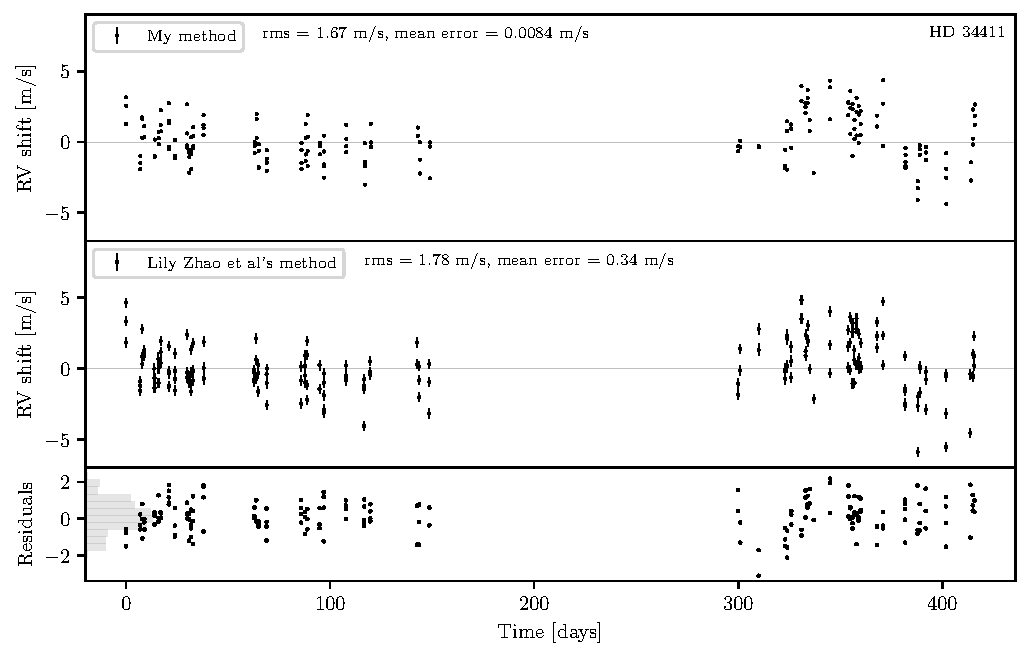
\includegraphics[width=\textwidth]{figures/HD34411_barycentric_rv_vs_lily.pdf}
        \caption{Top: my final extracted RV shifts for HD 34411 using Excalibur calibrated, barycentric-corrected data (data column \texttt{bary\char`_excalibur}). Center: Lily Zhao et al.'s results using a chunk-by-chunk (CBC) analysis technique \cite{yale_data}. Bottom: residuals from subtracting Zhao's results from mine. 188 observations made between 2019-10-8 and 2020-11-27.}
        \label{fig:HD34411_rvs}
    \end{wide}
\end{SCfigure}

It is likely that the very small errors are due to the interpolation done when calculating the individual feature cross-correlations. The errors get smaller with increasing number of sampled data points, $N$, and looking again at figure \ref{fig:err_vs_run_time} in appendix \ref{appendix:RV_extraction}, it appears that the error falls off as something like $1/\sqrt{N}$. A quick correction that one could make would thus be to "scale back" the errors by multiplying with $\sqrt{1000}$. Doing this, my mean error for HD 34411 comes out to $0.0084 \text{ m/s} \times \sqrt{1000} = 0.27$ m/s, which is about 20 \% off from the results of Zhao et al.

I have analyzed data from three more stars and again compared the results with those of Zhao et al. As with HD 34411, my rms values come within a few m/s, but the residuals are big and my errors are too small. Rescaling is an improvement. Results are summarized in table \ref{tabel:results}, while plots can be found in appendix \ref{appendix:results}.

\begin{SCtable}[1][!ht]%
    \begin{wide}  
        \resizebox{\textwidth}{!}{%
        \centering
        \begin{tblr}{
            @{}ccccccX[c,valign=b]X[c,valign=b]X[c,valign=b]@{}
        }
        \hline
            Star & RMS& RMS (Zhao)& RMS deviation & Mean error (scaled)& Mean error (Zhao)& Error deviation \\ \hline
            HD 34411 & 1.67 & 1.78 & -20.6 \% & 0.27 & 0.34 & -6.18 \% \\ \hline
            HD 101501 & 3.88 & 4.89 & -20.7 \% & 1.1 & 0.35 & 214 \% \\ \hline
            HD 10700 & 1.48 & 1.86 & -20.4 \% & 0.14 & 0.37 & -62.2 \% \\ \hline
            HD 26965 & 3.07 & 3.19 & -3.76 \% & 0.15 & 0.33 & -54.5 \% \\ \hline
        \end{tblr}}
        \caption{Summery of my results compared to those of Lily Zhao et al. All values listed are in m/s, except for the deviations, which are in percentage. Mean error (scaled) is the mean of the errors obtained from my method scaled by $\sqrt{1000}$.}
        \label{tabel:results}
    \end{wide}
\end{SCtable}
